\documentclass[a4paper,12pt]{article}
\usepackage[a4paper,top=1.3cm,bottom=2cm,left=1.5cm,right=1.5cm,marginparwidth=0.75cm]{geometry}
\usepackage{cmap}
\usepackage{mathtext}
\usepackage[T2A]{fontenc}
\usepackage[utf8]{inputenc}
\usepackage[english,russian]{babel}
\usepackage{siunitx}
\usepackage{enumitem}
\usepackage{placeins}

\usepackage{graphicx}
\usepackage{subcaption}
\usepackage{amsmath}

\usepackage{wrapfig}
\usepackage{tabularx}
\usepackage{multirow}

\usepackage{hyperref}
\usepackage[rgb]{xcolor}
\hypersetup{colorlinks=true,urlcolor=blue}
\usepackage{siunitx}
\usepackage{amsmath,amsfonts,amssymb,amsthm,mathtools}
\usepackage{mathtools}
\usepackage{icomma}
\mathtoolsset{showonlyrefs=false}
\usepackage{euscript}
\usepackage{mathrsfs}
\DeclareMathOperator{\sgn}{\mathop{sgn}}
\newcommand*{\hm}[1]{#1\nobreak\discretionary{}
{\hbox{$\mathsurround=0pt #1$}}{}}

%%% Заголовок
\newcommand\labname{Изучение спектров атомов водорода и дейтерия}
\newcommand\labnumber{2.2}


\author{Макаров Лев Евгеньевич}
\title{Лабораторная работа №\labnumber

\labname
}

\date{\today}

\makeatletter
\AddEnumerateCounter{\asbuk}{\russian@asbuk@alph}{щ} % section 8.1
\makeatother

\begin{document}

\begin{titlepage}
	\begin{center}
		{\large МОСКОВСКИЙ ФИЗИКО-ТЕХНИЧЕСКИЙ ИНСТИТУТ (НАЦИОНАЛЬНЫЙ ИССЛЕДОВАТЕЛЬСКИЙ УНИВЕРСИТЕТ)}
	\end{center}
	\begin{center}
		{\large Физтех-школа фотоники, электроники и молекулярной физики}
	\end{center}
	
	
	\vspace{4.5cm}
	{\huge
		\begin{center}
			{\bf Отчёт о выполнении лабораторной работы \labnumber}\\
			\labname
		\end{center}
	}
	\vspace{2cm}
	\begin{flushright}
		{\LARGE Автор:\\ Макаров Лев Евгеньевич \\
			\vspace{0.2cm}
			Б04-306}
	\end{flushright}
	\vspace{8cm}
	\begin{center}
		Долгопрудный 2025
	\end{center}
\end{titlepage}

\section{Введение}

\textbf{Цель работы:} 
\begin{enumerate}
	\item Исследовать энергетическую зависимость вероятности рассеяния электронов атомами ксенона;
    \item Определить энергии электронов, при которых наблюдается «просветление» ксенона;
    \item Оценить размер внешней электронной оболочки ксенона.
\end{enumerate}

\section{Теоретические сведения}

Эффективное сечение реакции (иногда его называют поперечным сечением или просто сечением реакции) — это величина, характеризующая вероятность перехода системы двух сталкивающихся частиц в результате их рассеяния (упругого или неупругого) в определенное конечное состояние.

\begin{equation}\label{eq:1}
    \sigma = \frac{N}{n v},
\end{equation}

где $N$ -- число переходов в единицу времени, $nv$ -- плотность потока рассеиваемых частиц.

\FloatBarrier
\begin{figure}[h]
    \begin{center}
        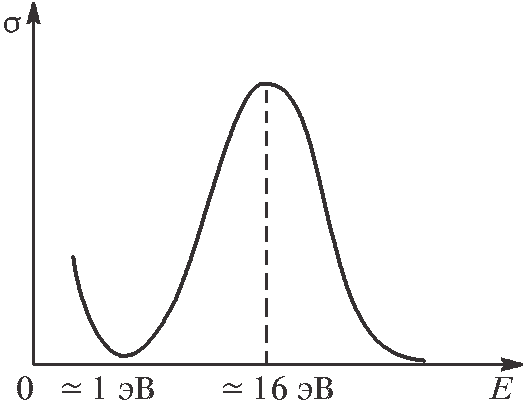
\includegraphics[width = 0.45\textwidth]{pics/ramzauer_qual.png}
        \caption{Качественная картина результатов измерения упругого рассеяния электронов в аргоне}
    \label{pic:ramzauer_qual}
    \end{center}
\end{figure}
\FloatBarrier

Качественно результат экспериментов Рамзауэра при энергии электронов порядка десятков электрон-вольт на аргоне показан на рис. \ref{pic:ramzauer_qual}.

По мере уменьшения энергии электрона от нескольких десятков электрон-вольт поперечное сечение его упругого рассеяния растет, как это и следует из очень простых рассуждений: чем меньше скорость электрона, тем медленнее он «проскакивает» мимо атома, тем больше время взаимодействия электронов с атомом и, тем самым, больше вероятность этого взаимодействия, т. е. сечение реакции. Однако в эксперименте наблюдалось, что при энергиях меньше 16 эВ сечение начинает уменьшаться, а при $E \simeq 1$ эВ практически равно нулю, т. е. аргон становится прозрачным для электронов. При дальнейшем уменьшении энергии электронов сечение рассеяния опять начинает возрастать.

Объяснение этого эффекта потребовало учета волновой природы электронов, что во времена становления квантовой механики в значительной степени способствовало укреплению новых физических воззрений на микромир. Схема эксперимента Рамзауэра показана на рис. \ref{pic:ustan_theor}.

\FloatBarrier
\begin{figure}[h]
    \begin{center}
        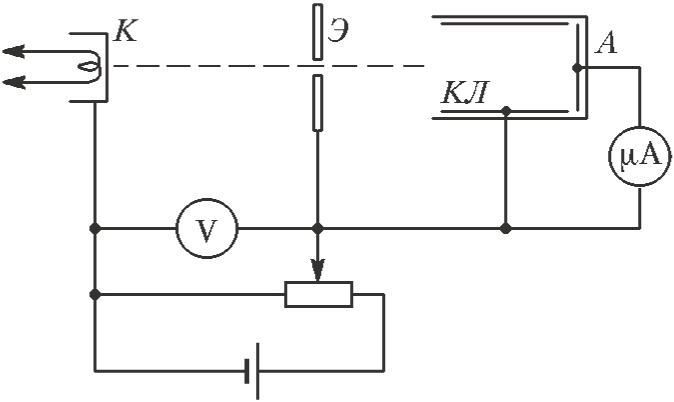
\includegraphics[width = 0.45\textwidth]{pics/ustan_theor.png}
        \caption{Схема установки для измерения сечения рассеяния электронов в газах}
    \label{pic:ustan_theor}
    \end{center}
\end{figure}
\FloatBarrier

Пучок электронов, вылетая из накаленного катода К, проходит ускоряющую разность потенциалов V , приложенную между катодом и электродом Э, и приобретает тем самым энергию $E = mv^2 /2 = eV$ . При прохождении через газ часть электронов рассеивается на атомах, уходит в сторону и собирается коллектором КЛ, а прошедшие без рассеяния электроны попадают на анод А и создают анодный ток $I$. Ток $I$ пропорционален числу прошедших электронов, и поэтому непосредственно характеризует проницаемость газа для электронного пучка в зависимости от его скорости (ускоряющего напряжения). Согласно классическим воззрениям с ростом напряжения $V$ , как указывалось выше, сечение рассеяния уменьшается, и ток должен монотонно возрастать.

С точки зрения квантовой теории картина рассеяния выглядит иначе. Внутри атома потенциальная энергия налетающего электрона $U$ отлична от нуля, скорость электрона изменяется, становясь равной $v'$ в соответствии с законом сохранения энергии

\begin{equation}\label{eq:2}
    E = \frac{mv^2}{2} = \frac{m v'^2}{2} + U,
\end{equation}

а значит, изменяется и длина его волны де Бройля. Таким образом, по отношению к электронной волне атом ведет себя как преломляющая среда с относительным показателем преломления

\begin{equation}\label{eq:3}
    n = \frac{\lambda}{\lambda'} = \sqrt{1 - \frac{U}{E}}.
\end{equation}

Решение задачи о рассеянии электрона на сферической потенциальной яме достаточно громоздко, поэтому мы для качественного анализа вопроса рассмотрим более грубую модель: будем считать, что электрон рассеивается на одномерной потенциальной яме конечной глубины. Форму реального потенциала для качественных оценок можно считать прямоугольной. Модель прямоугольной потенциальной ямы является хорошим приближением для атомов тяжелых инертных газов, отличающихся наиболее компактной структурой и резкой внешней границей.

Решение задачи о прохождении частицы с энергией $E$ над потенциальной ямой шириной $l$ и глубиной $U_0$ (рис. \ref{pic:shredinger_scheme}) можно найти во многих учебниках.

\begin{figure}[h]
    \begin{center}
        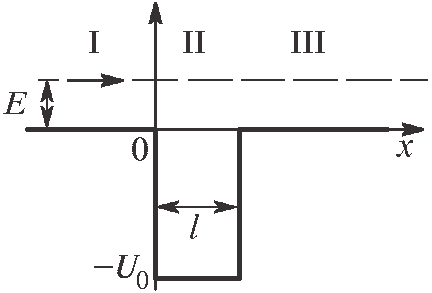
\includegraphics[width = 0.45\textwidth]{pics/shredinger_scheme.png}
        \caption{Схематическое изображение прямоугольной ямы, над которой пролетает частица с энергией $E$}
    \label{pic:shredinger_scheme}
    \end{center}
\end{figure}

Уравнение Шредингера в данном случае имеет вид

\begin{equation}\label{eq:4}
    \psi'' + k^2 \psi = 0, \ \text{где} \ k^2 = \begin{cases}
k_1^2 = \frac{2mE}{\hbar^2} - \ \text{в областях I и III};  \\
k_2^2 = \frac{2m\left(E + U_0\right)}{\hbar^2} - \ \text{в области II};  \\ 
\end{cases}
\end{equation}


Коэффициент прохождения равен отношению квадратов амплитуд прошедшей и падающей волн и определяется выражением

\begin{equation}\label{eq:5}
    D = \frac{16 k_1^2 k_2^2}{16 k_1^2 k_2^2 + 4\left(k_1^2 - k_2^2\right)^2 \sin^2 {\left(k_2 l\right)}}
\end{equation}

или

\begin{equation}\label{eq:6}
    D^{-1} = 1 + \frac{\left(k_1^2 - k_2^2\right)^2}{4 k_1^2 k_2^2} \sin^2 {\left(k_2 l\right)} = 1 + \frac{U_0^2}{4E \left(E + U_0\right)}\sin^2 {\left(k_2 l\right)}
\end{equation}

Мы видим, что коэффициент прохождения частицы над ямой имеет, в зависимости от ее энергии, ряд чередующихся максимумов и минимумов. В частности, если $k_2 l = \pi$, то $\sin \left(k_2 l\right) = 0$ и коэффициент прохождения равен единице, т. е. отраженная волна отсутствует, и электрон беспрепятственно проходит через атом, что является квантовым аналогом просветления оптики.

Таким образом, коэффициент прохождения электронов максимален при условии

\begin{equation}\label{eq:7}
    k_2 l = \sqrt{\frac{2m \left(E + U_0\right)}{\hbar^2}} l = n \pi, \ \ \ n=1,2,3,\ldots
\end{equation}

Это условие легко получить, рассматривая интерференцию электронных волн де Бройля в атоме. Движущемуся электрону соответствует волна де Бройля, длина которой определяется соотношением $\lambda = h/mv$. Если кинетическая энергия электрона невелика, то $E = mv^2/2$ и $\lambda = h / \sqrt{2mE}$. при движении электрона через атом длина волны де Бройля становится меньше и равна $\lambda' = h / \sqrt{2m\left(E + U_0\right)}$, где $U_0$ -- глубина атомного потенциала. При этом, как показано на рис. \ref{pic:atom_scheme}, волна де Бройля отражается от границ атомного потенциала, т. е. от поверхности атома, и происходит интерференция прошедшей через атом волны 1 и волны 2, отраженной от передней и задней границы атома (эти волны когерентны).

\begin{figure}[h]
    \begin{center}
        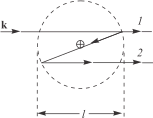
\includegraphics[width = 0.45\textwidth]{pics/atom_scheme.png}
        \caption{Схема интерференции волн де Бройля при рассеянии на атоме}
    \label{pic:atom_scheme}
    \end{center}
\end{figure}

Прошедшая волна 1 усилится волной 2, если геометрическая разность хода между ними $\Delta = 2l = \lambda'$ , что соответствует условию первого интерференционного максимума, т. е. при условии

\begin{equation}\label{eq:8}
    2l = \frac{h}{\sqrt{2m\left( E_1 + U_0 \right)}}
\end{equation}

Здесь $E_1$ — энергия электрона, соответствующая этому условию, которое естественно, совпадает с условием \eqref{eq:7}, следующим из решения уравнения Шредингера.

С другой стороны, прошедшая волна ослабится, если $\Delta = 2l = (3/2)\lambda'$ (условие первого интерференционного минимума), т. е. при условии

\begin{equation}\label{eq:9}
    2l = \frac{3}{2} \frac{h}{\sqrt{2m\left( E_2 + U_0 \right)}}
\end{equation}

Решая совместно эти два уравнения \eqref{eq:8} и \eqref{eq:9}, можно исключить $U_0$ и
найти эффективный размер атома $l$

\begin{equation}\label{eq:10}
    l = \frac{\sqrt{5}h}{\sqrt{32m\left( E_2 - E_1 \right)}}
\end{equation}

Понятно, что энергии $E_1$ и $E_2$ соответствуют энергиям электронов, прошедших разность потенциалов $V_1$ и $V_2$ , т. е. $E_1 = eV_1$ и $E_2 = eV_2$.

Из формул \eqref{eq:8} и \eqref{eq:9} можно также по измеренным величинам $E_1$ и $E_2$ рассчитать эффективную глубину потенциальной ямы атома:

\begin{equation}\label{eq:11}
    U_0 = \frac{4}{5} E_2 - \frac{9}{5} E_1.
\end{equation}

\section{Экспериментальная установка}

В данной работе для изучения эффекта Рамзауэра используется тиратрон ТГ3-01/1.3Б, заполненный инертным газом. Схематическое изображение тиратрона и его конструкция приведены на рис. \ref{pic:ustan}.

\begin{figure}[h]
    \begin{center}
        
\includegraphics[width = 0.45\textwidth]{pics/ustan.png}
        \caption{Схематическое изображение тиратрона (слева) и его конструкция (справа): 1, 2, 3 — сетки; 4 — внешний металлический цилиндр; 5 — катод; 6 — анод; 7 — накаливаемая спираль}
    \label{pic:ustan}
    \end{center}
\end{figure}

Электроны, эмитируемые катодом тиратрона, ускоряются напряжением $V$, приложенным между катодом и ближайшей к нему сеткой. Затем электроны рассеиваются на атомах инертного газа (ксенона). Все сетки 1, 2, 3 соединены между собой и имеют одинаковый потенциал, примерно равный потенциалу анода 6. Поэтому между первой сеткой 1 и анодом практически нет поля. Рассеянные электроны отклоняются в сторону и уходят на сетку, а оставшаяся часть электронов достигает анода и создает анодный ток $I_a$. Таким образом, поток электронов $N (x)$ на расстоянии $x$ от ускоряющей сетки (т. е. число электронов, проходящих через поперечное сечение лампы в точке $x$ в единицу времени) уменьшается с ростом $x$ от начального значения $N_0$ у катода (в точке $x = 0$) до некоторого значения $N_a$ у анода (в точке $x = L$).

Рассмотрим теперь, какова должна быть реальная вольт-амперная характеристика (ВАХ) тиратрона. Выделим в газе на расстоянии $x$ от катода тонкий слой с площадью поперечного сечения $S$ и толщиной $dx$ (см. рис. \ref{pic:ustan}). Этот слой содержит $d\nu = n_a Sdx$ атомов газа ($n_a$ — концентрация атомов газа в лампе). Суммарная рассеивающая поверхность этих атомов (суммарное эффективное сечение рассеяния) $\Delta = \nu \Delta_a$, где $\Delta_a$ — площадь поперечного сечения атома. Обозначим через $dN$ убыль потока электронов в результате прохождения слоя $dx$, тогда $dN/N (x)$ есть доля рассеянных электронов, или вероятность рассеяния в слое. Для рассеяния электрона в слое необходимо выполнение двух независимых событий — электрон должен «наткнуться» в слое на атом, и, кроме того, должен на этом атоме рассеяться. Следовательно, вероятность $dN/N (x)$ рассеяния электрона в слое равна произведению двух вероятностей — вероятности для электрона в слое $dx$ встретить атом газа (она равна $\Delta/S$ — доли площади поперечного сечения слоя, перекрываемого атомами) и вероятности рассеяния на атоме $w(V)$:

\begin{equation}\label{eq:12}
    - \frac{dN}{N(x)} = \frac{\Delta}{S} w(V) = n_a \Delta_a w(V) dx.
\end{equation}

Интегрируя это соотношение от 0 до $L$ и заменяя поток электронов на ток $I = N e$, получаем уравнение ВАХ:

\begin{equation}\label{eq:13}
    I_a = I_0 e^{- C w(V)}, \ \ \ C = L n_a \Delta_a,
\end{equation}

где $I_0 = eN_0$ -- ток катода, $I_a = eN_a$ -- анодный ток.

Согласно классическим представлениям сечение рассеяния электрона на атоме должно падать монотонно с ростом $V$ (обратно пропорционально скорости электрона, т. е. обратно пропорционально квадратному корню из его энергии), а значит, ВАХ будет монотонно возрастающей функцией, как это показано на рис. \ref{pic:electron_diffraction}а. По квантовым соображениям вероятность рассеяния электронов и соответствующая ВАХ должны иметь вид, показанный на рис. \ref{pic:electron_diffraction}б.

\begin{figure}[h]
    \begin{center}
        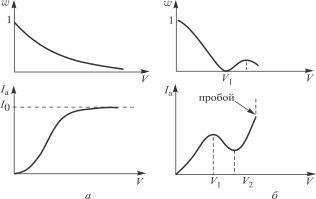
\includegraphics[width = 0.8\textwidth]{pics/electron_diffraction.png}
        \caption{Качественный вид вероятности рассеяния электрона атомом инертного газа и ВАХ тиратрона при классическом (a) и квантовом (б) рассмотрении}
    \label{pic:electron_diffraction}
    \end{center}
\end{figure}


Согласно формуле \eqref{eq:13} по измеренной ВАХ тиратрона можно определить зависимость вероятности рассеяния электрона от его энергии из соотношения

\begin{equation}\label{eq:14}
    w(V) = - \frac{1}{C} \ln \frac{I_a (V)}{I_0}
\end{equation}

\FloatBarrier
\section{Результаты измерений и обработка данных}


\subsection*{I. Подготовка приборов к работе}

\begin{enumerate}
    \item Установим все ручки регулировки на блоке питания в крайнее левое положение.
    \item Убедимся, что схема собрана корректно.
    \item Включим осциллограф в сеть.
    \item На канале I установим ступенчатый переключатель в режим 0.2 V/дел, утопим соседнюю кнопку $\times10$. Ручку плавного усиления повернем по часовой стрелке до щелчка.
    \item На канале II установим чувствительность 2 mV/дел$\times10$ = 20 mV/дел.
    \item Включим режим внешней развертки.
    \item Установим закрытый вход на обоих каналах ("$\sim$" на переключателе).
    \item Установим луч несколько правее от центра экрана.
    \item Убедимся, что напряжение накала подано на клеммы "общий" вольтметра.
\end{enumerate}

\subsection*{II. Измерения в динамическом режиме}

\begin{enumerate}
    \item Поставим переключатель на блоке питания в режим "ДИНАМИЧ".
    \item Установим напряжение накала лампы $U_\text{нак} = 2.85$ В.
    \item Проследим за ходом ВАХ тиратрона на экране ЭО при увеличении ускоряющего напряжения $U_{\text{катод–сетка}}$ от 0 до max. На характеристике видны максимум, минимум и начало второго максимума с переходом на пробой тиратрона.
    \item Перемещая сигнал ручками «$\leftrightarrow$» и «↑↓» и меняя чувствительность канала Y, добъемся размещения картины в центре экрана.
    \item При максимальном ускоряющем напряжении измерим на экране напряжения между катодом и сеткой, соответствующие первому максимуму и минимуму на осциллограмме. Запишем измерения в таблицу \ref{table:dynamic_Es}

\begin{table}[h]
    \centering
    \begin{tabular}{l|lll}
        \hline
        $U_{\text{нак}}$, В & $E_1$, В & $E_2$, В & $I_0$, мкА \\ \hline
        2.50             & 5.6      & 11.6     & 0.38       \\ 
        2.85             & 2.4      & 6.8      & 0.50       \\
        3.00             & 2.0      & 9.6      & 0.39       \\ \hline
    \end{tabular}
    \caption{Измерение напряжений в динамическом режиме}
    \label{table:dynamic_Es}
\end{table}


    \item Сохраним осциллограмму и изобразим на рис. \ref{pic:oscillograms}.

\begin{figure}[h!]
    \centering

    \begin{subfigure}[t]{0.31\textwidth}
        \centering
        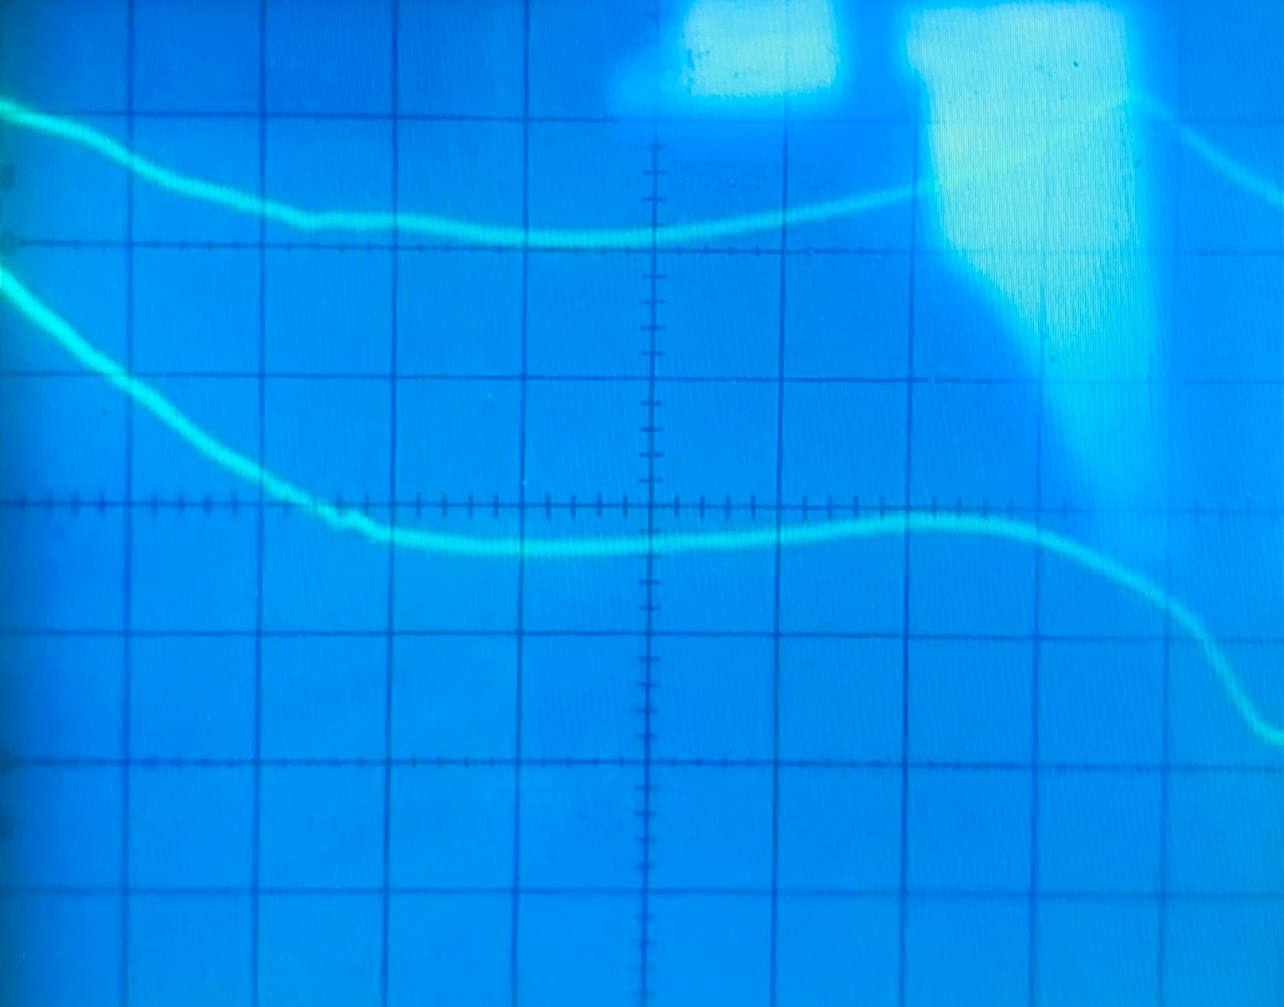
\includegraphics[width=\linewidth]{pics/oscilloscope_2.50.png}
        \caption{$U_{\text{нак}} = 2.50$ В}
        \label{pic:oscillogram_2_50}
    \end{subfigure}
    \hfill
    \begin{subfigure}[t]{0.31\textwidth}
        \centering
        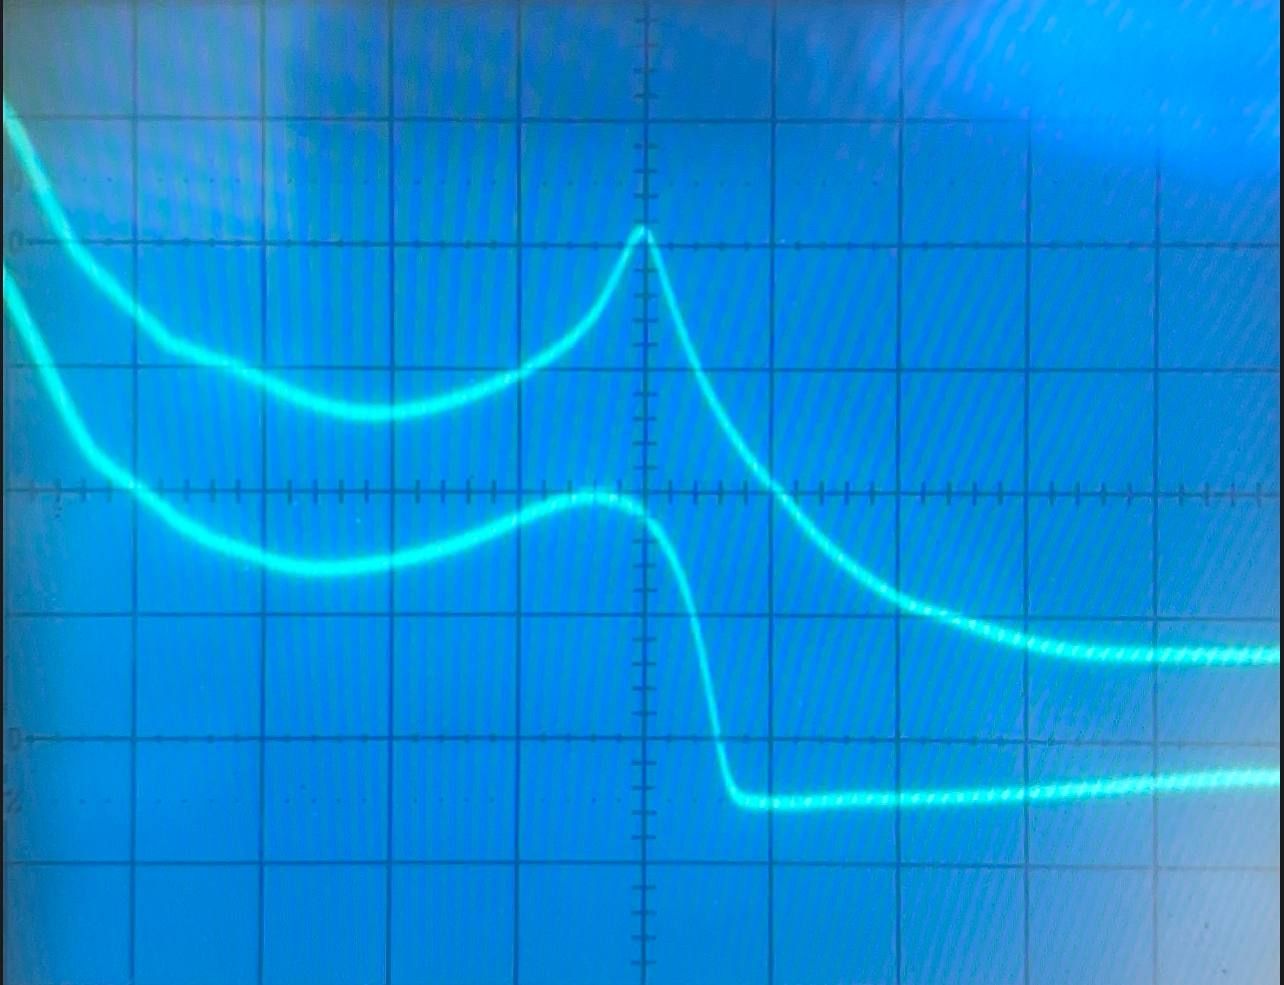
\includegraphics[width=\linewidth]{pics/oscilloscope_2.85.png}
        \caption{$U_{\text{нак}} = 2.85$ В}
        \label{pic:oscillogram_2_85}
    \end{subfigure}
    \hfill
    \begin{subfigure}[t]{0.31\textwidth}
        \centering
        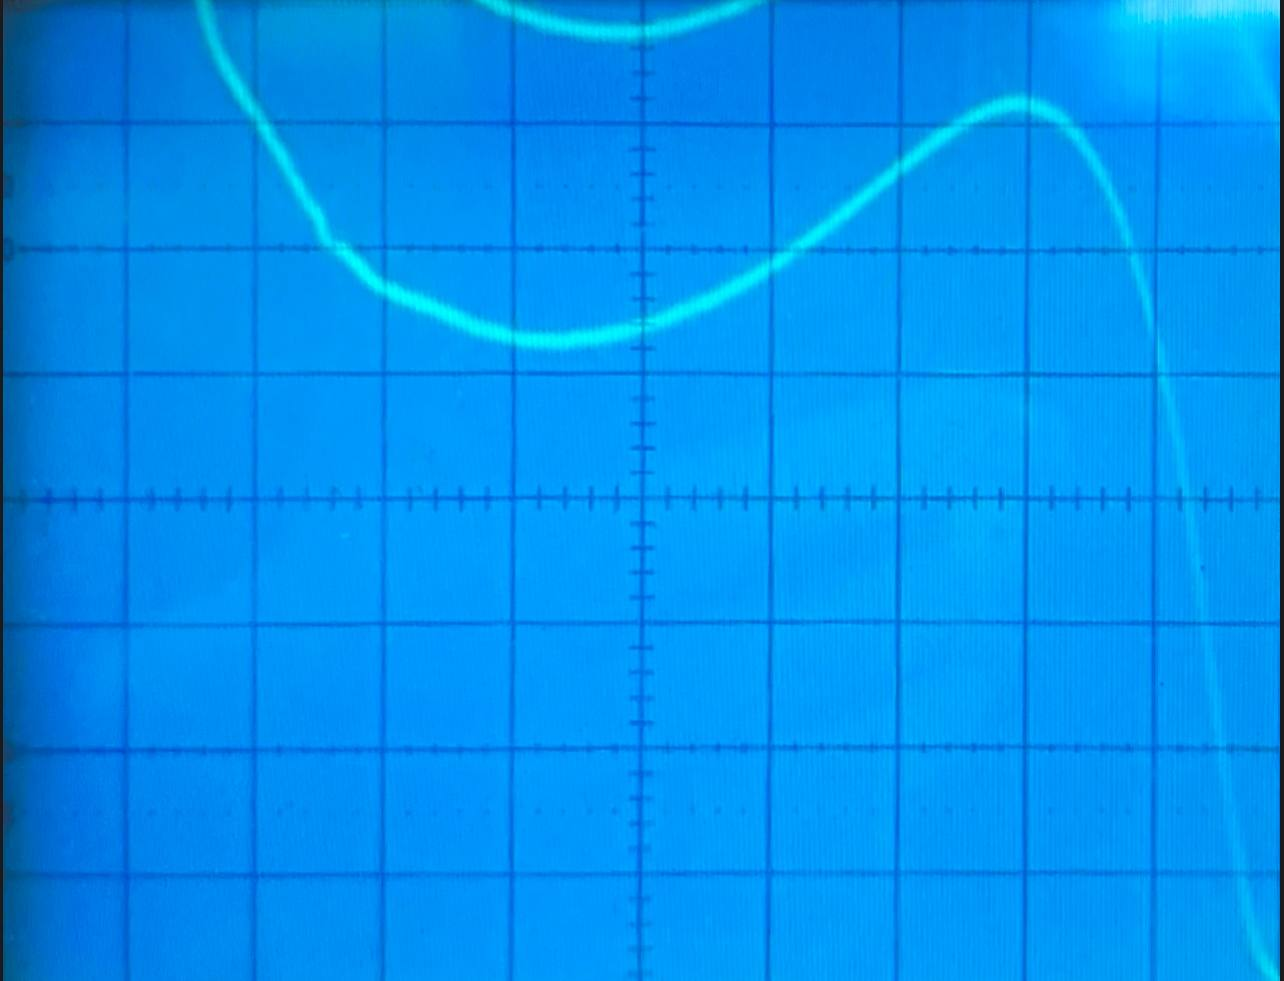
\includegraphics[width=\linewidth]{pics/oscilloscope_3.00.png}
        \caption{$U_{\text{нак}} = 3.00$ В}
        \label{pic:oscillogram_3_00}
    \end{subfigure}
    \caption{Три изображения в одном ряду}
    \label{pic:oscillograms}
\end{figure}

    \item Повторим измерения ВАХ тиратрона при напряжениях накала $U_\text{нак} = 2.50, 3.00$ В. Осциллограммы изобразим на рис. \ref{pic:oscillograms}.
    \item Поднесем к лампе постоянный магнит. Убедитесь, что это влияние магнита зависит от его ориентации относительно оси тиратрона.
    \item Выключите ЭО и вернем все ручки регулировки БИП на \textit{min}.
\end{enumerate}

\subsection*{III. Измерения в статическом режиме}

\begin{enumerate}
    \item Переведем переключатель на блоке питания в режим «СТАТИЧ».
    
    \item Убедимся, что напряжение «$V_{\text{катод–сетка}}$» подано на клеммы «0–1000~В» вольтметра, выберем режим измерения постоянного напряжения, диапазон — «20~В» и включим вольтметр в сеть.

    \item Убедимся, что сигнал с клемм $I_a$ подан на клеммы «0–2~В» вольтметра, выберем режим измерения постоянного напряжения (кнопки «–» и «V»), диапазон — «200~мВ» и включим вольтметр в сеть. Ток анода $I_a$ определяется по показанию вольтметра ($V_{\text{анод–сетка}}$), делённому на сопротивление $R = 100$ кОм, которое включено в цепь анода.

    \item Проведем измерение ВАХ тиратрона для двух значений напряжения накала $U_{\text{нак}} = 2.85, 3.00$ В.

    \item Установим ручку регулировки БИП на \textit{min} и отключим все приборы.
\end{enumerate}


\subsection*{IV. Обработка результатов}

\begin{enumerate}
    \item По результатам измерений в динамическом режиме рассчитаем размер электронной оболочки атома газа.
\end{enumerate}

\FloatBarrier
\begin{figure}[!ht]
	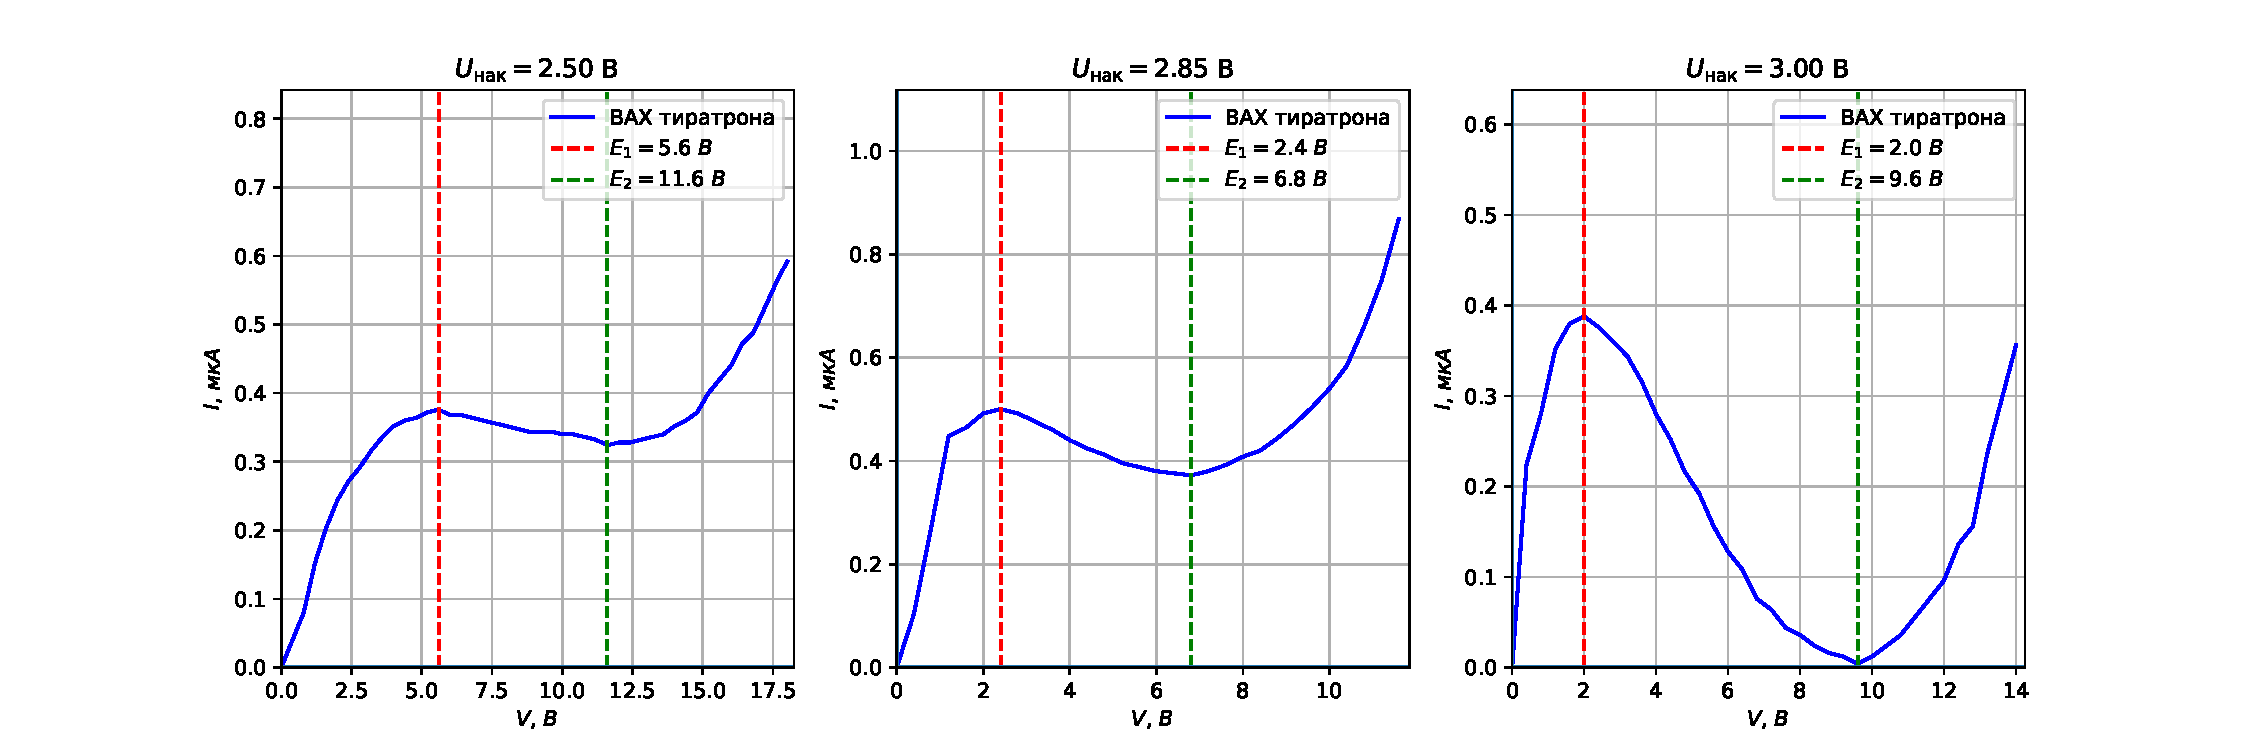
\includegraphics[width=1.1\textwidth]{plots/oscilloscopes_dynamic.pdf}
	\caption{\textit{ВАХ в динамическом режиме}}
	\label{pic:vah_dynamic}
\end{figure}
\FloatBarrier

Соотношения для размера:

\begin{equation*}
    2l = \cfrac{h}{\sqrt{2m \left(E_1 + U_0\right)}}, \ \ \ 2l = \cfrac{3}{2} \cfrac{h}{\sqrt{2m \left(E_2 + U_0\right)}}
\end{equation*}

В нашем случае положим $U_0 = 2.5$ В. Если выразить массу в эВ:

\begin{equation*}
    2l = \cfrac{h c}{\sqrt{2m \left(E_1 + U_0\right)}}, \ \ \ 2l = \cfrac{3}{2} \cfrac{hc}{\sqrt{2m \left(E_2 + U_0\right)}}
\end{equation*}

Если исключить $U_0$ (тоже масса в эВ):

\begin{equation*}
    l = \cfrac{hc \sqrt{5}}{\sqrt{32 m \left(E_2 - E_1\right)}}
\end{equation*}

Погрешности:

для вычисления через $E_1$ и $U_0$: 

\begin{equation*}
    \sigma_{1,0} = \left| \cfrac{\partial l}{\partial E_1} \right| \sigma_{E_1} = \left| - \cfrac{1}{4} \cfrac{hc \cdot 2m}{\sqrt{8m^3 \left(E_1 + U_0\right)^3}} \right| \sigma_{E_1} = \cfrac{hc\sigma_{E_1}}{4\sqrt{2m\left(E_1 + U_0\right)^3}} = l \cfrac{\sigma_{E_1}}{2(E_1 + U_0)}
\end{equation*}

для вычисления через $E_2$ и $U_0$: 

\begin{equation*}
    \sigma_{2,0} = \left| \cfrac{\partial l}{\partial E_2} \right| \sigma_{E_2} = \cfrac{3hc\sigma_{E_2}}{8\sqrt{2m\left(E_1 + U_0\right)^3}} = l \cfrac{\sigma_{E_2}}{2(E_2 + U_0)}
\end{equation*}

для вычисления через $E_1$ и $E_2$: 

\begin{multline*}
    \sigma_{1,2} = \sqrt{ \left( \cfrac{\partial l}{\partial E_1} \right)^2 \sigma_{E_1} + \left( \cfrac{\partial l}{\partial E_2} \right)^2 \sigma_{E_2} } = \\ = \sqrt{ \left( -\cfrac{1}{2} \cfrac{hc \sqrt{5} \cdot (-32m)}{\sqrt{32^3 m^3 \left(E_2 - E_1\right)^3}} \right)^2 \sigma_{E_1} + \left( -\cfrac{1}{2} \cfrac{hc \sqrt{5} \cdot (32m)}{\sqrt{32^3 m^3 \left(E_2 - E_1\right)^3}} \right)^2 \sigma_{E_2} } = \\ = \sqrt{ \left( \cfrac{1}{2} \cfrac{hc \sqrt{5}}{\sqrt{32 m \left(E_2 - E_1\right)^3}} \right)^2 \sigma_{E_1} + \left( \cfrac{1}{2} \cfrac{hc \sqrt{5}}{\sqrt{32 m \left(E_2 - E_1\right)^3}} \right)^2 \sigma_{E_2} } = \\= \sqrt{ \left( \cfrac{l}{2(E_2 - E_1)} \right)^2 \sigma_{E_1} + \left( \cfrac{l}{2(E_2 - E_1)} \right)^2 \sigma_{E_2} } = \cfrac{l\sqrt{\sigma_{E_1}^2 + \sigma_{E_2}^2}}{2(E_2 - E_1)}    
\end{multline*}

Посчитаем значения и их погрешности и запишем в таблицу \ref{table:sizes_dynamic}.


\begin{table}[h]
    \centering
    \begin{tabular}{l|ll|ll|ll}
        \hline
        $U_{\text{нак}}$, В & $l_{E_1}$, \AA & $\sigma_{l_{E_1}}$, \AA & $l_{E_2}$, \AA & $\sigma_{l_{E_2}}$, \AA & $l$, \AA & $\sigma_{l}$, \AA \\ \hline
        2.50 & 2.16 & 0.03 & 2.45 & 0.02 & 2.8 & 0.1 \\
        2.85 & 2.78 & 0.06 & 3.02 & 0.03 & 3.3 & 0.1 \\
        3.00 & 2.90 & 0.06 & 2.65 & 0.02 & 2.5 & 0.1 \\ \hline
    \end{tabular}
    \caption{Вычисление размера электронной оболочки}
    \label{table:sizes_dynamic}
\end{table}

\begin{enumerate}[resume]
    \item Оценим глубину потенциальной ямы по формуле \eqref{eq:11}. Запишем результаты вычислений в таблицу \ref{table:dynamic_U_0}
\end{enumerate}

\begin{equation*}
    U_0 = \frac{4}{5} E_2 - \frac{9}{5} E_1
\end{equation*}


\begin{table}[h]
    \centering
    \begin{tabular}{l|lll}
        \hline
        $U_{\text{нак}}$, В & 2.50 & 2.85 & 3.00 \\ \hline
        $U_0$, эВ           & -0.8 & 1.12 & 4.08 \\ \hline
    \end{tabular}
    \caption{Вычисление размера электронной оболочки}
    \label{table:dynamic_U_0}
\end{table}


\begin{enumerate}[resume]
    \item По полученным значениям определить газ невозможно, ведь они слишком разняться и явно не имеют смыла.
    \item Построим ВАХ для статического режима, изобразим его на рис. \ref{pic:static_vah}. Проведем те же рачеты, что и в динамическом режиме и запишем их в таблицу \ref{table:static}.
\end{enumerate}

\FloatBarrier
\begin{figure}[!ht]
	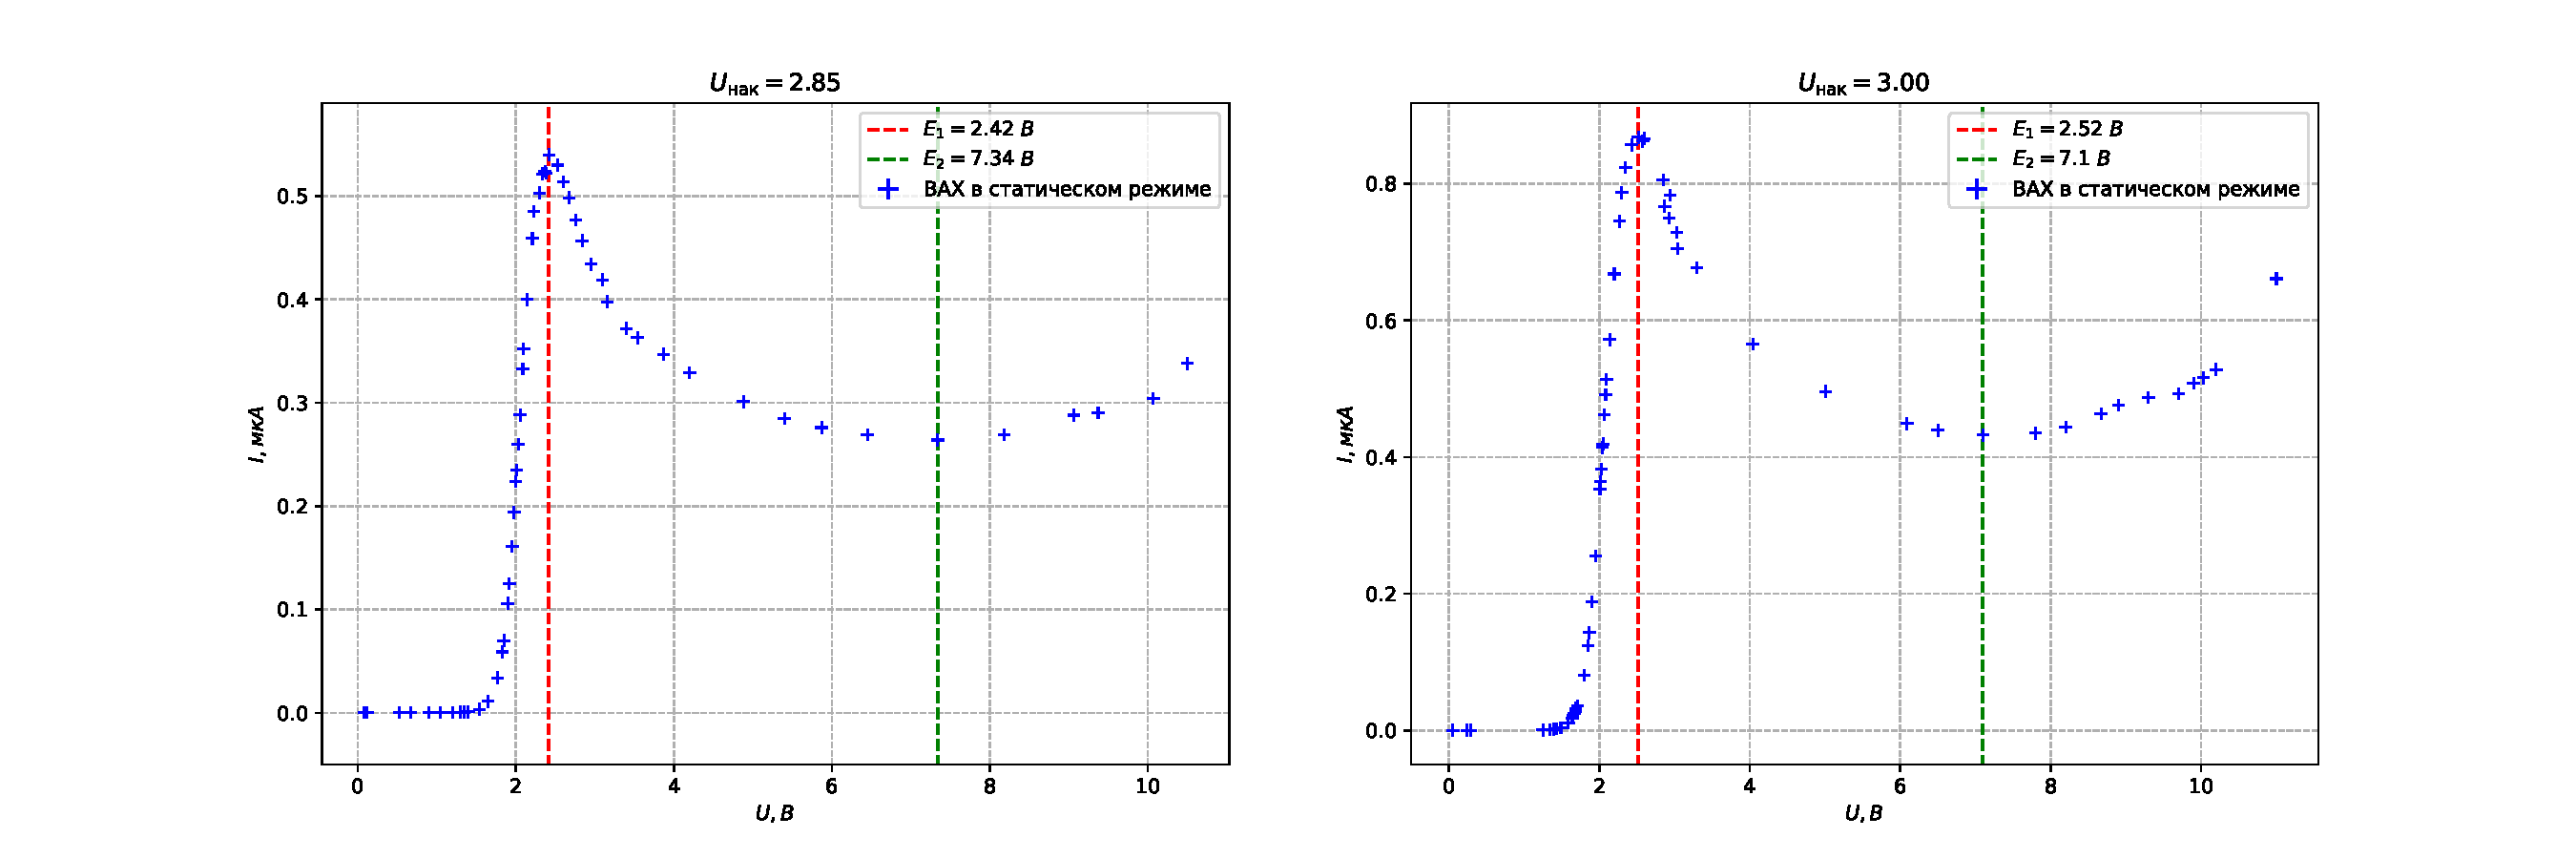
\includegraphics[width=1.1\textwidth]{plots/static_vah.pdf}
	\caption{\textit{ВАХ в статическом режиме режиме}}
	\label{pic:static_vah}
\end{figure}
\FloatBarrier


\begin{table}[h]
    \begin{tabular}{l|ll|l|ll|ll|ll|l|ll}
        \hline
        $U_{\text{нак}}$, В & $E_1$ & $E_2$, В & $I_0$, мкА & $l_{E_1}$ & $\sigma_{l_{E_1}}$, \AA & $l_{E_2}$ & $\sigma_{l_{E_2}}$, \AA & $l$ и $\sigma_{l}$, & \AA & $U_0$, эВ & $V_\text{проб}$ & $U_i$, В \\ \hline
        2.85 & 2.42 & 7.34 & 0.54 & 2.77 & 0.06 & 2.94 & 0.03 & 3.1 & 0.1 & 1.516 & 10.5 & 12.016 \\
        3.00 & 2.52 & 7.10 & 0.87 & 2.74 & 0.05 & 2.97 & 0.03 & 3.2 & 0.1 & 1.144 & 11.0 & 12.144 \\ \hline
    \end{tabular}
    \caption{Измерения в статическом режиме}
    \label{table:static}
\end{table}

По полученному потенциалу пробоя можно сделать вывод, что тиратрон заполнен ксеноном.

\begin{enumerate}[resume]
    \item Используя формулу \eqref{eq:7}, оценим при каких напряжениях должны появляться максимумы в коэффициенте прохождения для электронов $n = 2, 3$.
\end{enumerate}

\begin{equation*}
    \sqrt{\cfrac{2m \left( E_n + U_0 \right)}{\hbar^2}} l = n \pi, \ \ \  \sqrt{\cfrac{2m \left( E_1 + U_0 \right)}{\hbar^2}} l = \pi \implies
\end{equation*}

\begin{equation*}
    \implies \cfrac{E_n + U_0}{E_1 + U_0} = n^2 \implies E_n = n^2 \left(E_1 + U_0\right) - U_0
\end{equation*}


\begin{table}[!h]
    \centering
    \begin{minipage}{0.48\textwidth}
        \centering
        \begin{tabular}{l|lll}
            \hline
            ~            & $E_1$, В & $E_2$, В & $E_3$, В \\ \hline
            эксперимент  & 2.42     & 7.34     & ~        \\
            предсказание & 2.42     & 13.67    & 32.42    \\ \hline
        \end{tabular}
        \caption{$U_{\text{нак}} = 2.85$ В}
    \end{minipage}
    \hfill
    \begin{minipage}{0.48\textwidth}
        \centering
        \begin{tabular}{l|lll}
            \hline
            ~            & $E_1$, В & $E_2$, В & $E_3$, В \\ \hline
            эксперимент  & 2.52     & 7.10     & ~        \\
            предсказание & 2.52     & 14.07    & 33.32    \\ \hline
        \end{tabular}
        \caption{$U_{\text{нак}} = 3.00$ В}
    \end{minipage}
    \label{table:grad}
\end{table}

\begin{enumerate}[resume]
    \item Найдем зависимость вероятности рассеяния электрона от энергии и построим график. Для статического режима на рис. \ref{pic:static_w} и на рис. \ref{pic:dynamic_w} для динамического режима.
\end{enumerate}

\begin{equation*}
    w(V) = - \cfrac{1}{C} \ln {\cfrac{I_a(V)}{I_0}}
\end{equation*}

\FloatBarrier
\begin{figure}[!ht]
	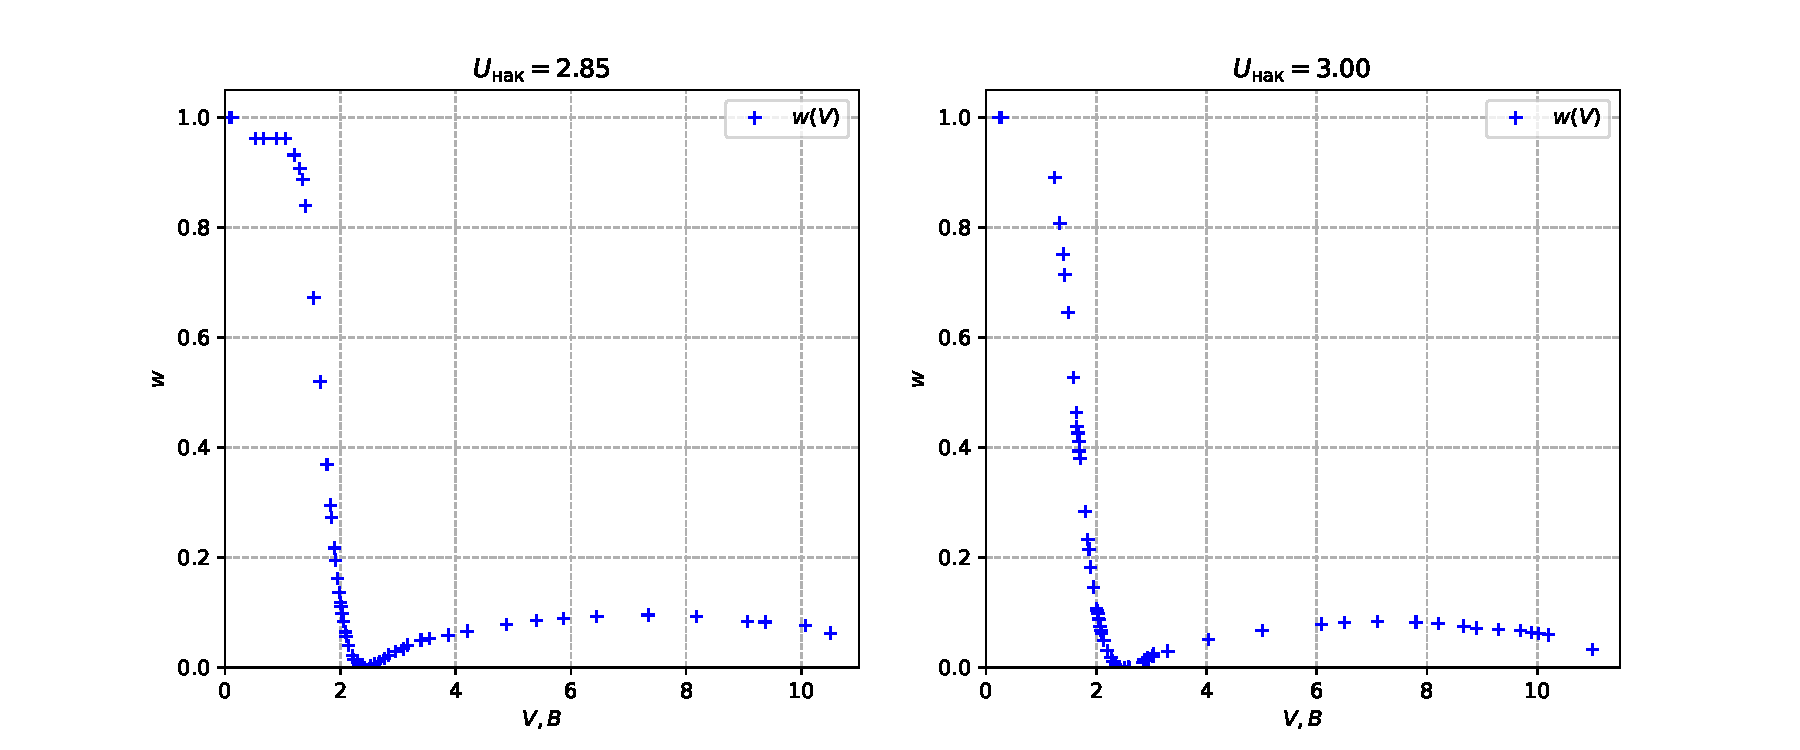
\includegraphics[width=1.1\textwidth]{plots/w_static.pdf}
	\caption{\textit{$w(V)$ в статическом режиме}}
	\label{pic:static_w}
\end{figure}
\FloatBarrier

\FloatBarrier
\begin{figure}[!ht]
	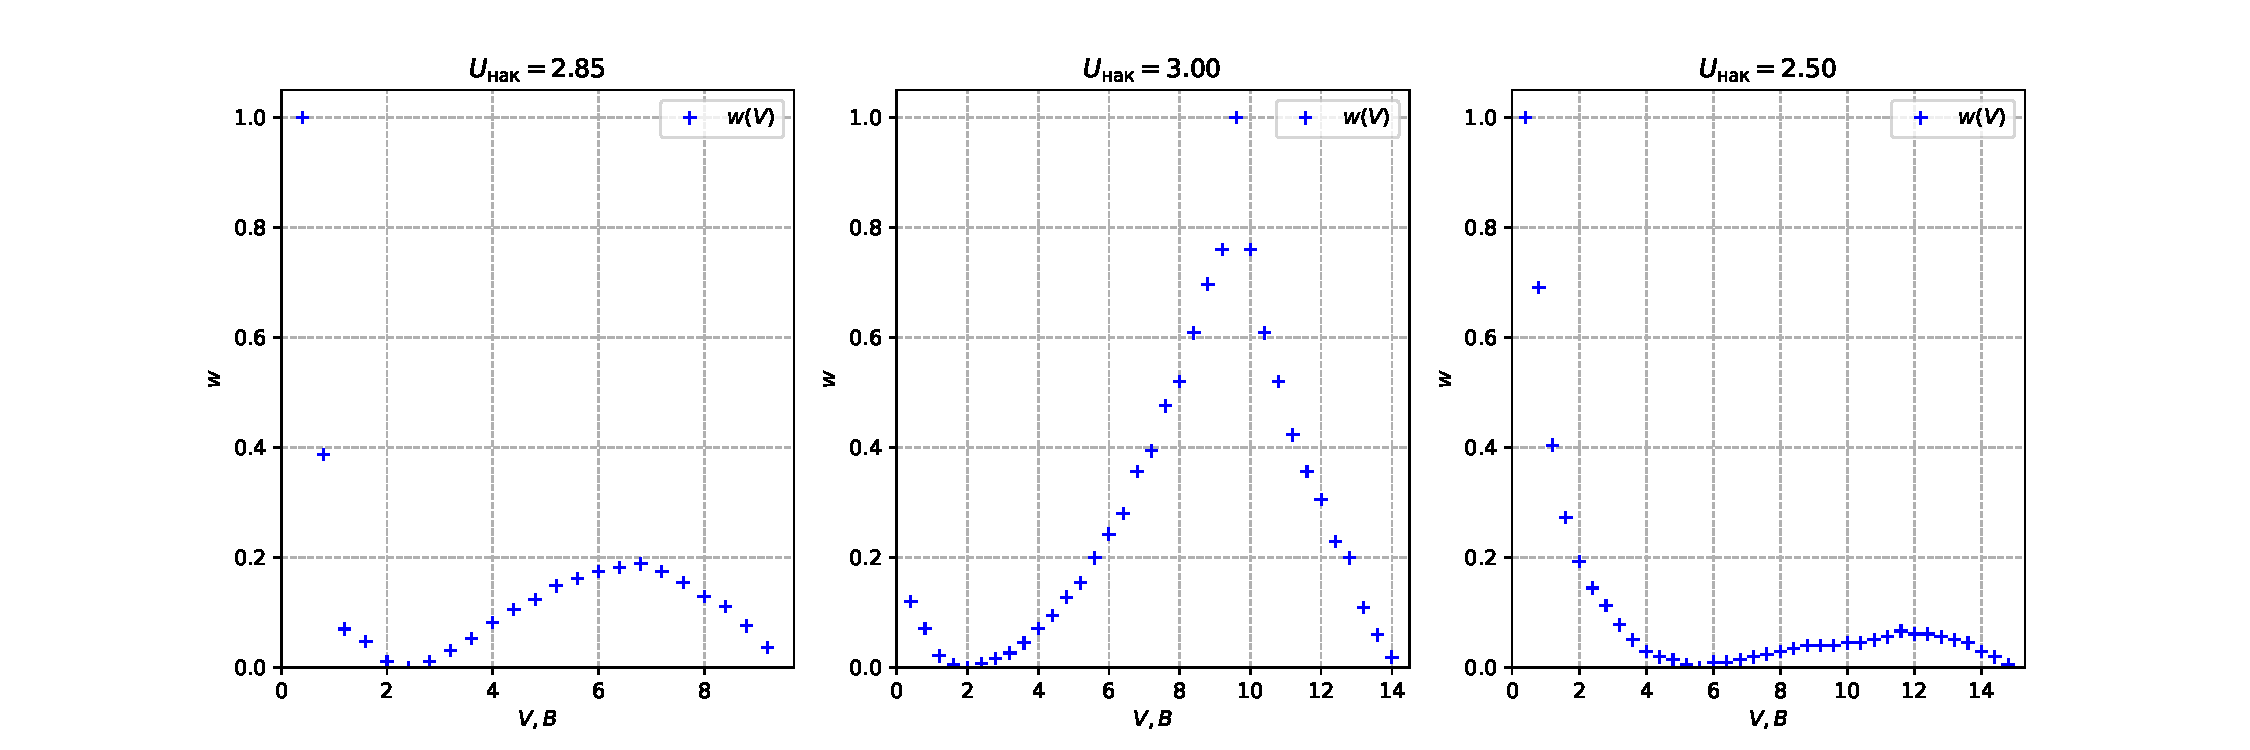
\includegraphics[width=1.1\textwidth]{plots/w_dynamic.pdf}
	\caption{\textit{$w(V)$ в динамическом режиме}}
	\label{pic:dynamic_w}
\end{figure}
\FloatBarrier

\section{Выводы}

\begin{enumerate}
    \item Исследована энергетическая зависимость вероятности рассеяния электрона атомами ксенона. Определены минимумы и максимумы. Посчитан потенциал ионизации.
    \item Определен размер электронной оболочки атома ксенона.
\end{enumerate}


\end{document}
